\section{Eigenvalue problem}
This section is devoted to the approximate solution of the eigenvalue problem, needed for the Schr\"odinger equation \eqref{eq:spe_ks}. 
\\Eigenvalue problems are ubiquitous in physics and engineering, and while solving one for a small matrix is trivial, it still requires roughly $O(n^3)$ operations \cite{golub13} to do so. More often than not, real computational applications result in large-scale matrices, which are completely out of question for exact eigenvalues calculations, thus requiring the use of approximate algorithms. 
\\We will begin by describing common building blocks of iterative eigensolvers in section \ref{sec:techniques}, namely:
\begin{itemize}
    \item the approximate solutions of linear systems by the use of the Conjugate Gradient method;
    \item matrix preconditioning to speed up convergence;
    \item the Rayleigh-Ritz procedure to find good approximations to the eigenpairs in a certain subspace; and
    \item the shift-and-invert method, to select the desired portion of the eigenvalue spectrum.
\end{itemize}
After describing these building blocks, some of the most commonly used eigensolvers are described in section \ref{sec:eigensolvers}, focusing on the core ideas and stating their limitations, to finally address the General Conjugate Gradient method, whose implementation in the present work is detailed in section \ref{sec:gcg}.
\subsection{Conjugate Gradient and numerical techniques}
\label{sec:techniques}
\subsubsection{Conjugate Gradient method}
\label{sec:cg}
Solving linear systems of the form
\begin{equation}
    \label{eq:lin_sys}
    Ax = b
\end{equation}
is crucial in many eigensolvers. The Conjugate Gradient (CG) is perhaps the most famous iterative solver in this sense, especially in connection with sparse matrices, as we will see in a moment.
CG applies to cases where $A$ is a real, $n\times n$, positive-definite, symmetric matrix, and $x$ and $b$ are $n$-dimensional vectors.
\\Many generalizations to this method exist, which relax the requirements on the matrix, like BiCGSTAB, CGRES and so on \cite{Saad1992}. We will describe the working principle of CG, but the same applies to all the others, with slight variations.
\paragraph{Steepest descent method}
The quadratic form $f(x)$ derived from the system \eqref{eq:lin_sys} is
\begin{equation}
    \label{eq:quad_form}
    f(x) = \frac 1 2 x^T A x - b^T x
\end{equation}
If $A$ is symmetric, positive-definite, the shape of $f(x)$ is convex and has a global minimum for
\begin{equation}
    \label{eq:quad_form_min}
    \nabla_x f(x) = A x_m - b = 0 \implies A x_m = b,
\end{equation}
hence the extremum of the quadratic form is the also the solution of the linear system \eqref{eq:lin_sys}.
\\We can employ the well-known gradient descent technique \cite{PainlessCGM} to find such point: starting from a guess $x_0$, we compute the direction $d_i$ where $f$ decreases the most (the residual $r_i$), compute the step size that gives the largest decrease, and update $x_i$ at each iteration accordingly, repeating until convergence.
\begin{align}
d_i = r_i &= b - A x_i \\
x_{i+1} &= x_i +\alpha_i r_i \\
\text{with } \alpha_i \text{ such that } \dv{f}{\alpha_i} = 0 \implies \alpha_i &= \frac{r_i^T r_i}{r_i^T A r_i}
\end{align}
This is a powerful but highly inefficient procedure. We are not ensuring that the search direction doesn't end up with components in subspaces that were explored already.
\\It can be proven \cite{PainlessCGM} that the norm of the error $e_i = x_i - x_m$ is minimal at each iteration if the search directions $d_i$ are chosen to be $A$-orthogonal to the next error, i.e. $d_i^T A e_{i+1} = 0$. This makes the algorithm converge at the exact solution in $n$ steps, but most importantly it allows to truncate the iterations without a large error on the approximation $x_i$.
\\In this case, the algorithm is called Conjugate Gradient Method and is formulated as 
\begin{align}
    \label{eq:cg_method}
    \alpha_i = \frac{r_i^T r_i}{d_i^T A d_i}  
    \\x_{i+1} = x_i + \alpha_i d_i
    \\r_{i+1} = r_i - \alpha_i A d_i
    \\\beta_{i+1} = \frac{r_{i+1}^T r_{i+1}}{r_i^T r_i}
    \\d_{i+1} = r_{i+1} + \beta_{i+1} d_i
\end{align}
where iterations are truncated if the norm of the residual $r_i$ is smaller than a certain threshold. It can be proven that the orthonormalization of the new search direction, with respect to all the previous ones, can be done only through the rescaling factor $\beta_{i+1}$ \cite{PainlessCGM}.
CG converges to the exact solution in $n$ steps, moreover, it represents a great method for sparse matrices, because it can be proven to be of complexity $O(m)$, where $m$ is the number of non-zero elements in $A$ \cite{PainlessCGM}. In figure \ref{fig:cg}, a visual representation of the conjugation of search directions and the subsequent exact solution is shown for a two-dimensional problem.
\begin{figure}[h]
\centering
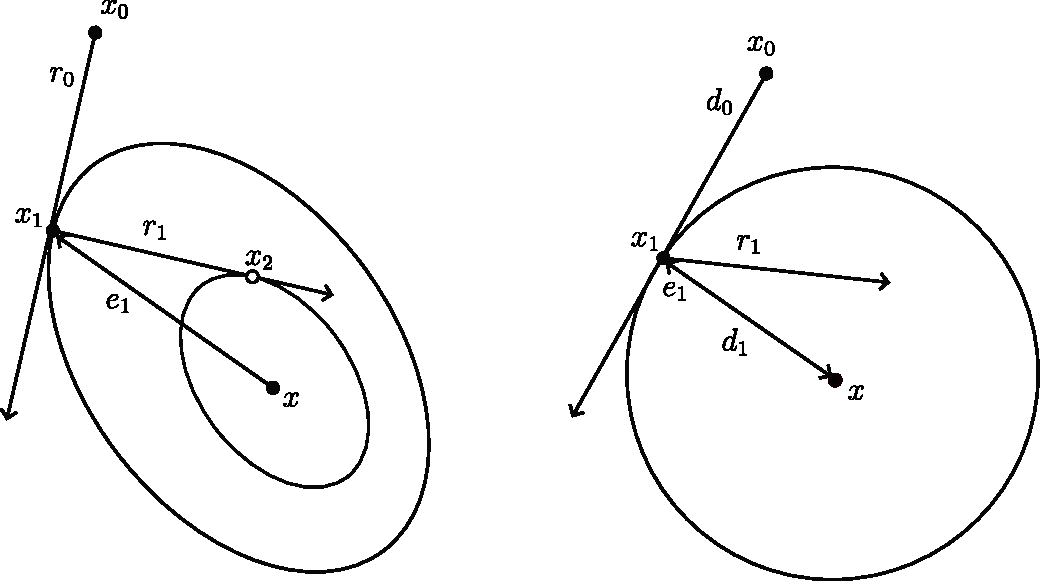
\includegraphics[width=0.8\textwidth]{Images/cg}
\caption{Comparison between the steepest descent method, on the left, and the conjugate gradient method, on the right, for a two-dimensional matrix. Ellipses represent contour lines of the quadratic form $f(x) = x^T A x - b^T x$, in the `stretched' space $Ax$ on the right. As shown in the figure, the conjugation of the search directions eliminates components of the error $e_i$, until the exact convergence in $n$ (2) steps.}
\label{fig:cg}
\end{figure}
\paragraph{Complex matrices} Algorithm \eqref{eq:cg_method} and the CG method in general can be used for complex matrices, under the condition that $A$ is Hermitian and positive-definite when using the complex inner product, meaning that
\begin{equation}
    A = A^\dagger\text{ and }
    x^\dagger Ax > 0.
\end{equation}
\subsubsection{Preconditioning}
\label{sec:preconditioning}
The CG method convergence is known to be limited by the modulus of the condition number of $A$, $\kappa(A)$, given by \cite{PainlessCGM}
\begin{equation}
    \label{eq:cond_num}
    \kappa(A) = \frac{\lambda_\text{max}(A)}{\lambda_\text{min}(A)}
\end{equation}
where $\lambda_\text{max}$ and $\lambda_\text{min}$ are respectively the largest and smallest eigenvalues of $A$ in magnitude.
If we were able to find a good \textit{preconditioner} $M$, symmetric and positive-definite, such that $\kappa(M^{-1}A) \lll \kappa(A)$, and $M^{-1}$ is easy to compute, then the algorithm would converge much faster, by solving $M^{-1}Ax = M^{-1}b$, since $x$ is also the solution of $Ax = b$.
\begin{equation}
    \label{eq:precond}
    x = (M^{-1}A)^{-1} M^{-1}b = A^{-1} MM^{-1} b = A^{-1} b.
\end{equation}
Without delving into the details of the preconditioner implementation, detailed in \cite{PainlessCGM}, note that, in general, $M^{-1}A$ is neither positive-definite nor symmetric, which requires a Cholesky decomposition \cite{cholesky} $M = EE^T$ to be used, so that the problem may be restated with a symmetric positive-definite matrix $E^{-1}AE^{-T}$.
\\The catch with preconditioning is that $M$ has no unique recipe. Preconditioners are widely spread across numerical analysis, so many methods have been explored and implemented \cite{pearson2020preconditioners}.
\subsubsection{Rayleigh-Ritz procedure}
\label{sec:rayleigh_ritz}
A common denominator of all these algorithms is the search of good approximations for the correct eigenvectors in a certain subspace. The method is called Rayleigh-Ritz (RR) procedure \cite{Saad1992}, and is here outlined.
\\Let us suppose to have a matrix $A$ of size $n\times n$, with entries in $\C$ and a collection of vectors $k$ organized in a matrix $K$, where $K$ is of size $n\times k$. Generally speaking, $n$ is large, while $k$ is much smaller.
\\The best approximation of the true eigenvectors of $A$ in the subspace $\mathcal K$ spanned by the vectors in $K$ can be computed by solving the small scale eigenvalue problem
\begin{equation}
    K^\dagger A  K C = C\Lambda.
\end{equation}
Here matrices $K^\dagger A K$ and $C$ are of size $k\times k$.
Computing $K C$ gives a matrix of size $n\times k$, whose column vectors are the best approximations of the true eigenvectors of $A$ in the subspace  $\mathcal K$, with their corresponding eigenvalues in the entries of the diagonal matrix $\Lambda$.
\subsubsection{Shift and Invert}
\label{sec:shift_invert}
The power iteration is the technique on which Krylov subspace search methods are based \cite{golub13}. By repeatedly applying matrix $A$ to a vector $x$, $x$ gets skewed towards the eigenvector whose eigenvalue is of largest magnitude $\lambda_n$.
\\Let us assume $A$ is a hermitian matrix, thus diagonalizable. This means we can write an arbitrary vector $x^{(0)}$ as a linear combination of the eigenvectors $\{v_i\}$ of $A$.
\begin{equation}
    x^{(0)} = \sum_i^n \alpha_i v_i
\end{equation}
If we apply $A$ to $x^{(0)}$ k times, we get
\begin{equation}
    x^{(k)} = A^k x^{(0)} = \sum_i^n \alpha_i A^k v_i = \sum_i^n \alpha_i\lambda_i ^{k}v_i
\end{equation}
It can be proven that the ratio of the $j$-th component of $x_j^{(k)}$ and $x_j^{(k-1)}$ converges to $\lambda_n$
\begin{equation}
    \label{eq:power_iter_ratio}
    \lim_{k\to\infty} \frac{x_j^{(k)}}{x_j^{(k-1)}} = \lambda_n
\end{equation}
which means, that for large enough $k$, we have the relation
\begin{equation}
    \label{eq:power_iter_lambda}
    A x^{(k)} \approx \lambda_n x^{(k)}
\end{equation}
So $x^{(k)}$ is an approximation of the eigenvector $v_n$ of $A$ whose eigenvalue is $\lambda_n$.
\paragraph{Smallest eigenvalue}
If instead of the largest eigenvalue, we were interested in the smallest one -- in magnitude -- $\lambda_0$, then we would need to apply the inverse matrix $A^{-1}$ to $x^{(k)}$, which would change the ratio \eqref{eq:power_iter_ratio} to 
\begin{equation}
    \label{eq:power_iter_ratio_inv}
    \lim_{k\to\infty} \frac{x_j^{(k)}}{x_j^{(k-1)}} = \lambda_0
\end{equation}
Let us assume for a moment that we're solving a nuclear single-particle Hamiltonian, where we have a certain number of bound states of negative energy and a much larger number of unbound states with positive energy. In this case, the inverse power iteration would converge to the states whose energy is closer to zero, avoiding the interesting ones on the bottom of the spectrum.
\\The solution is, before inverting, to shift the matrix by a quantity $\sigma$ that is very close to the lowest eigenvalue we want to compute, call it $\lambda_\sigma$ (eigenvector $v_\sigma$).
Now, the eigenvalue of lowest magnitude of $(A-\sigma I)$ is $\lambda_\sigma - \sigma$ and by applying $(A-\sigma I)^{-1}$ to $x^{(k)}$, we will get the approximation to the eigenvector $v_\sigma$. This is the procedure implemented in step \ref{alg:inv_pow_step} of algorithm \ref{alg:mod_gcg}.
\subsection{Iterative eigensolvers}
\label{sec:eigensolvers}
Now that the main techniques used by iterative eigensolvers have been laid out, we can look at three general methods, which are the most commonly used ones.
\subsubsection{Jacobi-Davidson}
The Jacobi-Davidson method is a type of algorithm where at each iteration, the approximation to an eigenpair of matrix $A$, is improved by correcting the eigenvector through the solution of a certain linear system, as we shall see shortly.
\\Given an approximation $(u, \theta)$ of an eigenpair of matrix $A$, where $u$ is the approximate eigenvector and $\theta$ is the approximate eigenvalue, if the residual
\begin{equation}
    \label{eq:residual}
    r= A u - \theta u
\end{equation}
is $\approx 0$, then the eigenpair converged. Otherwise, we want to find a correction $t$ such that 
\begin{equation}
    \label{eq:jacobi_correction}
    r= A(u+t) - (\theta + \delta \theta) (u+t) = 0 
\end{equation}
Linearizing this equation in $t$ gives
\begin{equation}
   (A - \theta  I ) t = -r 
\end{equation}
To avoid singularity of the equation near convergence, since $u$ approximately spans a subspace of the system's kernel $\text{ker} (A-\theta I)$, and enrich the subspace search with a useful orthogonal correction, we project the problem onto the orthogonal subspace of $u$, which finally gives
\begin{equation}
    \label{eq:jacobi_eq_proj}
    ( I - uu^\dagger) (A - \theta  I )(I - u u^\dagger) t = -r
\end{equation}
\begin{algorithm}[h]
\caption{Jacobi-Davidson method}
\begin{algorithmic}[1]
\STATE Choose normalized initial vectors $\{u_k\}$, set $V = [u_1, \ldots, u_{k}]$
\REPEAT
    \STATE Compute eigenpair: $T = V^\dagger A V$, solve $T y = \theta y$
    \STATE Set $u = V y$, residual $r = A u - \theta u$
    \IF{$\|r_k\| < \varepsilon\ \forall k$}
         \RETURN $(\theta, u)$
    \ENDIF
    \STATE Solve approximately $(I - u_k u_k^\dagger)(A - \theta I)(I - u_k u_k^\dagger) t_k = -r_k$
        using preconditioned iterative solver, ensuring $t_k \perp u_k$
    \STATE Normalize: $v_k = t_k / \|t_k\|$
    \STATE Expand subspace, setting $V = [V, v]$
\UNTIL{convergence}
for $k = 1, \dots, \text{nev}$
\end{algorithmic}
\end{algorithm}
Although simple, this method is computationally efficient only by using preconditioning, which is known to be unstable in many cases \cite{Saad1992}.
\subsubsection{Lanczos}
Lanczos algorithm \cite{lanczos1952solution} is probably the most used iterative eigensolver for hermitian matrices. It's a Krylov subspace search method, meaning the Rayleigh-Ritz procedure is done on a subspace formed as 
\begin{equation}
    \mathcal K = \{ v_1, Av_1, A^2 v_1, \ldots, A^{k-1} v_1 \}
\end{equation}
which exploits the power iteration. After orthogonalizing the new approximation to the previous one and diagonalizing the small scale problem, we end up with the new best approximations to the eigenvectors of $A$.
\begin{algorithm}[h]
\caption{Lanczos Method}
\begin{algorithmic}[1]
\STATE Choose normalized initial vector $v_1$, set $\beta_0 = 0$, $m=$ subspace size.
\REPEAT
\FOR{$j = 1, 2, \dots, m$}
    \STATE $w \gets A v_j - \beta_{j-1} v_{j-1}$
    \STATE $\alpha_j \gets v_j^* w$
    \STATE $w \gets w - \alpha_j v_j$
    \STATE $\beta_j \gets \|w\|$
    \IF{$\beta_j = 0$}
        \STATE \textbf{break}
    \ENDIF
    \STATE $v_{j+1} \gets w / \beta_j$
\ENDFOR
\STATE Form tridiagonal matrix 
       $T_m = \mathrm{tridiag}(\beta_{1:m-1}, \alpha_{1:m}, \beta_{1:m-1})$
\STATE Compute eigen-decomposition $T_m y_k = \theta_k y_k$, 
       for $k = 1, \dots, \text{nev}$
\STATE Form Ritz approximations 
       $x_k = V_m y_k$, where $V_m = [v_1, \dots, v_m]$
\STATE Compute residual norms 
       $r_k = \|A x_k - \theta_k x_k\|$ for all $k$
\UNTIL convergence for $k = 1, \dots, \text{nev}$
\end{algorithmic}
\end{algorithm}
Lanczos is extremely efficient, memory- and CPU-wise for extremal eigenvalues, but this limits its applicability, as one may be interested in the inner portion of the eigenvalue spectrum, such in the case of Hartree-Fock-Bogoliubov (HFB).
\\A shift-and-invert strategy would be unfeasible in the case of large scale problems, since all Lanczos steps need to be performed exactly to avoid instabilities, a well known problem in the Arnoldi generalization \cite{Saad1992}.
\subsubsection{LOBPCG}
The last algorithm of this short list is LOBPCG, it's the newest and most sophisticated one of the three.
\\Introduced by A. V. Knyazev in 1991 \cite{LOBPCG}, it's a block, preconditioned conjugate gradient method, explicitly targeted at solving large-scale eigenvalue problems, and it has been used in modern solutions of the Schr\"odinger/KS equation in recent years \cite{LOBPCGDKS,Nottoli2023,LIN2013205,li2020efficient}.
\\We won't go into the details of LOBPCG, since GCG shares with it many aspects, like blocking and search directions calculation.
\\LOBPCG works very well for large scale problems, but it has limitations. 
On the one hand, it's not possible to arbitrarily select the portion of the matrix spectrum to calculate, which is required for problems where variational collapse happens, like in HFB or the Dirac equation, which manifests particle/antiparticle solutions \cite{li2020efficient}.
To solve this, an additional filtering step is required \cite{LIN2013205,li2020efficient}, which introduces a computational cost in the algorithm.
\\Lastly, LOBPCG may fail when poor conditioning is present or when high precision on the eigenvalues is required \cite{GCG1}.
\subsection{General Conjugate Gradient}
\label{sec:gcg}
The General Conjugate Gradient is an iterative eigensolver designed with the aim of improving LOBPCG, it is a blocked algorithm, which uses the inverse power method and previous search directions to generate the search subspace. GCG is proven to be faster and more stable than LOBPCG \cite{GCG1}.
\\The search subspace is built as
\begin{equation}
    V = [X, P, W],
\end{equation}
where $X$, of dimensions $n\times k$ is the matrix containing the approximations, to the eigenvectors of matrix $A$, $P$, of dimensions $n\times k$ is the matrix containing the previous search directions, and $W$, of dimension $n\times a$ is the matrix containing the eigenvectors on which the inverse power method is applied approximately using the CG.
\\A slightly different implementation of the algorithm is employed in the present work, detailed in algorithm \ref{alg:mod_gcg}, to improve applicability to HF calculations and reduce the computational cost.
\paragraph{Eigenvalue problem} The original algorithm aims at solving the general eigenvalue problem $AX = \lambda BX$. Since in our case $B=I$, it is omitted from the procedure, reducing the computational cost of the algorithm, in particular, the one of the search direction block $P$. After orthonormalization of $V$, the columns of $X$ are orthonormal as well and the calculation of $P$ is given by
\begin{equation}
    \label{eq:gcg_p}
    P = X_\text{new} - X(X^\dagger X_\text{new})
\end{equation}
which is the projection of $X_\text{new}$ onto the orthogonal complement of $X$, used in step \ref{alg:directions} of algorithm \ref{alg:mod_gcg}.
\paragraph{Complex matrix} The algorithm has been generalized to the complex case, where the matrix is complex Hermitian and, as such, the transposition operation is replaced by the conjugate transpose.
\paragraph{Blocking} The algorithm is designed to allow blocking of the eigenvectors, such that $X=[X_c, X_a, X_r]$, where $X_c$ are the converged eigenvectors, $X_a$ are the active eigenvectors on which we perform the inverse power iteration, with $\text{col}(X_a)$ being a fixed number, and $X_r$ are the remaining eigenvectors, which are to be inserted in $X_a$ as soon as some of its columns converge. This allows to save some computations by avoiding the expensive inverse power on pairs that have already converged. Since in a self-consistent calculation the matrix changes rapidly at each HF iteration, it is the case that the maximum number of iterations is reached before convergence of all eigenpairs, so we must work at all times on the remaining unconverged eigenvectors. For this reason, we only implement the $X=[X_c, X_a]$ scheme, where the only distinction we make is between converged eigenvectors $X_c$ and unconverged ones $X_a$.
\paragraph{Orthogonalization} The original paper \cite{GCG1} suggests an improved orthogonalization procedure; being beyond the scope of this work, the simpler Gram-Schmidt \cite{GM} orthogonalization is used in the present work.
\paragraph{Shift update} The shift update is either fixed, in case of known spectrum, eg for HFB $\texttt{shift} = 0$, or adaptive \cite{GCG1}, so that the inverse power step can find the lowest eigenvalues, using the update formula
\begin{equation}
    \label{eq:update_shift}
    \texttt{shift}=(\lambda_\text{nev} - 100\lambda_1)/99
\end{equation}
where $\lambda_\text{nev}$ is the biggest eigenvalue of the RR procedure and $\lambda_1$ is the smallest of the active eigenpairs.
\paragraph{Preconditioning} The use of a preconditioner is beyond the scope of this work, a simple diagonal preconditioner is used.
\begin{algorithm}[h]
\caption{General Conjugate Gradient algorithm}
\begin{algorithmic}[1]
    \label{alg:mod_gcg}
\STATE \textbf{Input:} Matrix \(A\) of dimensions $n\times n$, number of desired eigenpairs \( \texttt{nev} \), $X_\text{guess}$ initial guess of dimensions $n\times k$, with $= k \ge \text{nev}$, \(\texttt{max\_iter}\) maximum iterations
\STATE Initialize block $X=[ X_\text{a}]$ $\gets X_\text{guess}$ and $X_c$ as an empty block
\STATE Initialize blocks \( P \) and \( W \) as empty blocks
\STATE Solve the Rayleigh Ritz problem \(X^\dagger A X C= C \Lambda \)
\STATE Update \(X=X C\)
\STATE Initialize $\texttt{shift}$, Initialize $\texttt{iter} = 0$ 
\WHILE{$\text{col}(X_c) < \texttt{nev}$ and $\texttt{iter} < \texttt{max\_iter}$}
    \STATE Solve approximately \( (A+ \texttt{shift}\cdot I)W = X_a\Lambda \) with some CG steps, initial value $X_a$ to generate W as an approximation to $W = (A+\texttt{shift}\cdot I)^{-1}X_a\Lambda$ \label{alg:inv_pow_step} 
    \STATE Orthogonalize \( V=[X, P, W] \), of dimensions $n\times (k+k+a)$
    \STATE Solve the Rayleigh Ritz problem \(V^\dagger (A + \texttt{shift}\cdot I) V C= C\Lambda \)
    \STATE Update \(X_\text{new}\) with the first $\texttt{nev}$ columns of $VC$ and \(\Lambda_\text{new} = \Lambda - \texttt{shift}\cdot I\)
    \STATE Compute \(P=X_\text{new} - X(X^\dagger X_\text{new})\) \label{alg:directions}
    \STATE Compute the residual \( R = AX_\text{new} - \Lambda X_\text{new} \) 
    \STATE Check convergence on $k$-th column norm of \(R\), if $\|R_k\| < \texttt{tol}$, move \(X_{a,k}\) to \(X_c\).
    \STATE Update $\texttt{shift}$ using formula \eqref{eq:update_shift} and $\texttt{iter}\gets \texttt{iter} + 1$
\ENDWHILE
\STATE \textbf{Output:} Approximate eigenpairs \( (\Lambda, X) \)
\end{algorithmic}
\end{algorithm}

